Class templates may also have a variable number of template arguments. This is key to building some categories of types, such as tuple and variant, that are available in the standard library. In this section, we will see how we could write a simple implementation for a tuple class. A tuple is a type that represents a fixed-size collection of heterogeneous values.

When implementing variadic function templates we used a recursion pattern with two overloads, one for the general case and one for ending the recursion. The same approach has to be taken with variadic class templates, except that we need to use specialization for this purpose. Next, you can see a minimal implementation for a tuple:

\begin{lstlisting}[style=styleCXX]
template <typename T, typename... Ts>
struct tuple
{
	tuple(T const& t, Ts const &... ts)
	: value(t), rest(ts...)
	{
	}

	constexpr int size() const { return 1 + rest.size(); }
	
	T value;
	tuple<Ts...> rest;
};

template <typename T>
struct tuple<T>
{
	tuple(const T& t)
	: value(t)
	{
	}

	constexpr int size() const { return 1; }
	
	T value;
};
\end{lstlisting}

The first class is the primary template. It has two template parameters: a type template and a parameter pack. This means, at the minimum, there must be one type specified for instantiating this template. The primary template tuple has two member variables: value, of the T type, and rest, of type tuple<Ts…>. This is an expansion of the rest of the template arguments. This means a tuple of N elements will contain the first element and another tuple; this second tuple, in turn, contains the second element and yet another tuple; this third nested tuple contains the rest. And this pattern continues until we end up with a tuple with a single element. This is defined by the partial specialization tuple<T>. Unlike the primary template, this specialization does not aggregate another tuple object.

We can use this simple implementation to write code like the following:

\begin{lstlisting}[style=styleCXX]
tuple<int> one(42);
tuple<int, double> two(42, 42.0);
tuple<int, double, char> three(42, 42.0, 'a');

std::cout << one.value << '\n';
std::cout << two.value << ','
          << two.rest.value << '\n';
std::cout << three.value << ','
          << three.rest.value << ','
          << three.rest.rest.value << '\n';
\end{lstlisting}

Although this works, accessing elements through the rest member, such as in three.rest.rest.value, is very cumbersome. And the more elements a tuple has the more difficult it is to write code in this way. Therefore, we'd like to use some helper function to simplify accessing the elements of a tuple. The following is a snippet of how the previous could be transformed:

\begin{lstlisting}[style=styleCXX]
std::cout << get<0>(one) << '\n';
std::cout << get<0>(two) << ','
          << get<1>(two) << '\n';
std::cout << get<0>(three) << ','
          << get<1>(three) << ','
          << get<2>(three) << '\n';
\end{lstlisting}

Here, get<N> is a variadic function template that takes a tuple as an argument and returns a reference to the element at the N index in the tuple. Its prototype could look like the following:

\begin{lstlisting}[style=styleCXX]
template <size_t N, typename... Ts>
typename nth_type<N, Ts...>::value_type & get(tuple<Ts...>& t);
\end{lstlisting}

The template arguments are the index and a parameter pack of the tuple types. Its implementation, however, requires some helper types. First, we need to know what the type of the element is at the N index in the tuple. This can be retrieved with the help of the following nth\_type variadic class template:

\begin{lstlisting}[style=styleCXX]
template <size_t N, typename T, typename... Ts>
struct nth_type : nth_type<N - 1, Ts...>
{
	static_assert(N < sizeof...(Ts) + 1,
	              "index out of bounds");
};

template <typename T, typename... Ts>
struct nth_type<0, T, Ts...>
{
	using value_type = T;
};
\end{lstlisting}

Again, we have a primary template that uses recursive inheritance, and the specialization for the index 0. The specialization defines an alias called value\_type for the first type template (which is the head of the list of template arguments). This type is only used as a mechanism for determining the type of a tuple element. We need another variadic class template for retrieving the value. This is shown in the following listing:

\begin{lstlisting}[style=styleCXX]
template <size_t N>
struct getter
{
	template <typename... Ts>
	static typename nth_type<N, Ts...>::value_type&
	get(tuple<Ts...>& t)
	{
		return getter<N - 1>::get(t.rest);
	}
};

template <>
struct getter<0>
{
	template <typename T, typename... Ts>
	static T& get(tuple<T, Ts...>& t)
	{
		return t.value;
	}
};
\end{lstlisting}

We can see here the same recursive pattern, with a primary template and an explicit specialization. The class template is called getter and has a single template parameter, which is a non-type template parameter. This represents the index of the tuple element we want to access. This class template has a static member function called get. This is a variadic function template. The implementation in the primary template calls the get function with the rest member of the tuple as an argument. On the other hand, the implementation of the explicit specialization returns the reference to the member value of the tuple.

With all these defined, we can now provide an actual implementation for the helper variadic function template get. This implementation relies on the getter class template and calls its get variadic function template:

\begin{lstlisting}[style=styleCXX]
template <size_t N, typename... Ts>
typename nth_type<N, Ts...>::value_type &
get(tuple<Ts...>& t)
{
	return getter<N>::get(t);
}
\end{lstlisting}

If this example seems a little bit complicated, perhaps analyzing it step by step will help you better understand how it all works. Therefore, let's start with the following snippet:

\begin{lstlisting}[style=styleCXX]
tuple<int, double, char> three(42, 42.0, 'a');
get<2>(three);
\end{lstlisting}

We will use the cppinsights.io web tools to check the template instantiations that occur from this snippet. The first to look at is the class template tuple. We have a primary template and several specializations, as follows:

\begin{lstlisting}[style=styleCXX]
template <typename T, typename... Ts>
struct tuple
{
	tuple(T const& t, Ts const &... ts)
	   : value(t), rest(ts...)
	{ }
	
	constexpr int size() const { return 1 + rest.size(); }
	
	T value;
	tuple<Ts...> rest;
};

template<> struct tuple<int, double, char>
{
	inline tuple(const int & t,
	             const double & __ts1, const char & __ts2)
	: value{t}, rest{tuple<double, char>(__ts1, __ts2)}
	{}
	
	inline constexpr int size() const;
	
	int value;
	tuple<double, char> rest;
};

template<> struct tuple<double, char>
{
	inline tuple(const double & t, const char & __ts1)
	: value{t}, rest{tuple<char>(__ts1)}
	{}
	
	inline constexpr int size() const;
	
	double value;
	tuple<char> rest;
};

template<> struct tuple<char>
{
	inline tuple(const char & t)
	: value{t}
	{}
	
	inline constexpr int size() const;
	
	char value;
};

template<typename T>
struct tuple<T>
{
	inline tuple(const T & t) : value{t}
	{ }
	
	inline constexpr int size() const
	{ return 1; }
	
	T value;
};
\end{lstlisting}

The tuple<int, double, char> structure contains an int and a tuple<double, char>, which contains a double and a tuple<char>, which, in turn, contains a char value. This last class represents the end of the recursive definition of the tuple. This can be conceptually represented graphically as follows:

\begin{center}
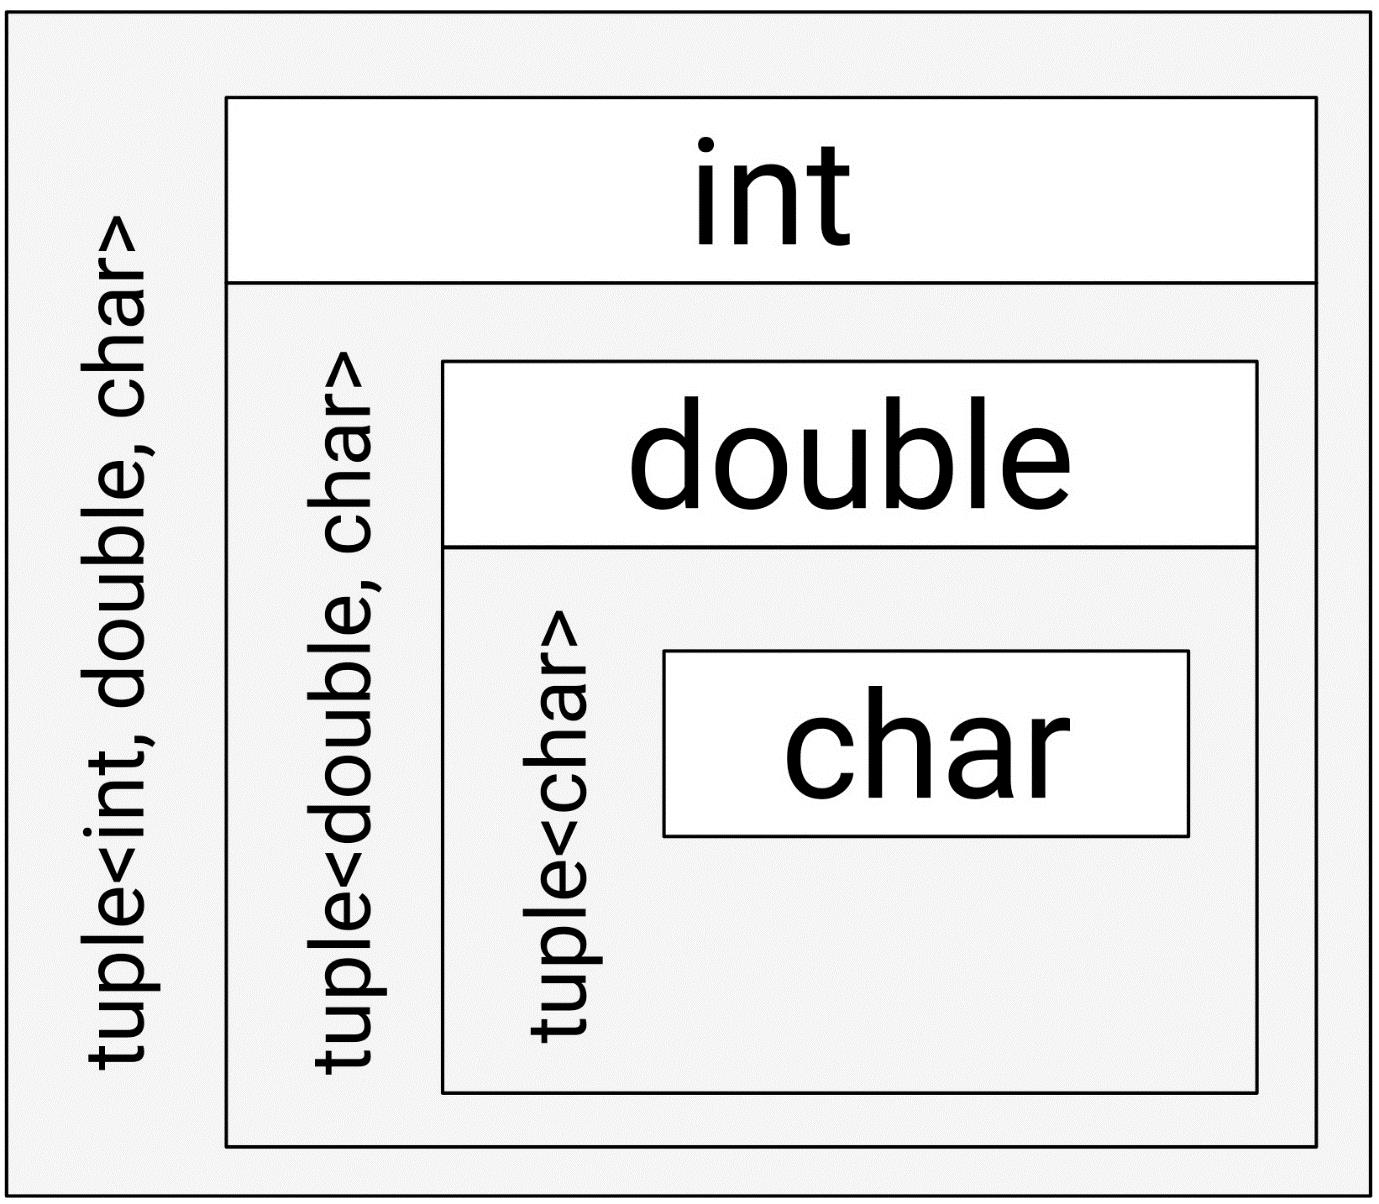
\includegraphics[width=0.4\textwidth]{content/1/chapter3/images/1.png}\\
Figure 3.1 – An example tuple
\end{center}

Next, we have the nth\_type class template, for which, again, we have a primary template and several specializations, as follows:

\begin{lstlisting}[style=styleCXX]
template <size_t N, typename T, typename... Ts>
struct nth_type : nth_type<N - 1, Ts...>
{
	static_assert(N < sizeof...(Ts) + 1,
	              "index out of bounds");
};

template<>
struct nth_type<2, int, double, char> :
   public nth_type<1, double, char>
{ };

template<>
struct nth_type<1, double, char> : public nth_type<0, char>
{ };

template<>
struct nth_type<0, char>
{
	using value_type = char;
};

template<typename T, typename ... Ts>
struct nth_type<0, T, Ts...>
{
	using value_type = T;
};
\end{lstlisting}

The nth\_type<2, int, double, char> specialization is derived from nth\_type<1, double, char>, which in turn is derived from nth\_type<0, char>, which is the last base class in the hierarchy (the end of the recursive hierarchy).

The nth\_type structure is used as the return type in the getter helper class template, which is instantiated as follows:

\begin{lstlisting}[style=styleCXX]
template <size_t N>
struct getter
{
	template <typename... Ts>
	static typename nth_type<N, Ts...>::value_type&
	get(tuple<Ts...>& t)
	{
		return getter<N - 1>::get(t.rest);
	}
};

template<>
struct getter<2>
{
	template<>
	static inline typename
	nth_type<2UL, int, double, char>::value_type &
	get<int, double, char>(tuple<int, double, char> & t)
	{
		return getter<1>::get(t.rest);
	}
};

template<>
struct getter<1>
{
	template<>
	static inline typename nth_type<1UL, double,
	                                char>::value_type &
	get<double, char>(tuple<double, char> & t)
	{
		return getter<0>::get(t.rest);
	}
};
template<>
struct getter<0>
{
	template<typename T, typename ... Ts>
	static inline T & get(tuple<T, Ts...> & t)
	{
		return t.value;
	}

	template<>
	static inline char & get<char>(tuple<char> & t)
	{
		return t.value;
	}
};
\end{lstlisting}

Lastly, the get function template that we use to retrieve the value of an element of a tuple is defined as follows:

\begin{lstlisting}[style=styleCXX]
template <size_t N, typename... Ts>
typename nth_type<N, Ts...>::value_type &
get(tuple<Ts...>& t)
{
	return getter<N>::get(t);
}

template<>
typename nth_type<2UL, int, double, char>::value_type &
get<2, int, double, char>(tuple<int, double, char> & t)
{
	return getter<2>::get(t);
}
\end{lstlisting}

Should there be more calls to the get function more specializations of get would exist. For instance, for get<1>(three), the following specialization would be added:

\begin{lstlisting}[style=styleCXX]
template<>
typename nth_type<1UL, int, double, char>::value_type &
get<1, int, double, char>(tuple<int, double, char> & t)
{
	return getter<1>::get(t);
}
\end{lstlisting}

This example helped us demonstrate how to implement variadic class templates with a primary template for the general case and a specialization for the end case of the variadic recursion.

You have probably noticed the use of the keyword typename to prefix the nth\_type<N, Ts...>::value\_type type, which is a dependent type. In C++20, this is no longer necessary. However, this topic will be addressed in detail in Chapter 4, Advanced Template Concepts.

Because implementing variadic templates is often verbose and can be cumbersome, the C++17 standard added fold expressions to ease this task. We will explore this topic in the next section.


